\section{Control of Robotic Systems}

\subsection{Controlling a robot}

\textbf{Definition:} Determine, through appropriate algorithms, the control inputs that ensure the robot behaves as desired both kinematically (position/velocity) and dynamically (forces, interaction).

Before designing the control algorithms it is useful to clarify some preliminary aspects: what constitutes the control input of the robot (\textbf{actuation}), how the control system is structured (\textbf{architecture}), how the desired behavior is defined (\textbf{planning}), and how robust operation is guaranteed (\textbf{stability}).

\hfill

\subsection{Actuation}

Every joint is actuated by a \textbf{servomotor}. Depending on the application, the actuator may be pneumatic or hydraulic—capable of delivering very high payloads but offering limited control flexibility and slow motion—or an \textbf{electrical motor}, which enables precise trajectory tracking and high control flexibility at the cost of payload capacity.
    
The most commonly used electrical servomotors are DC motors with permanent magnets and brushless motors. \textit{Remember that we control the motors to control the robot.}

\newpage

\subsubsection*{Servomotor}

\begin{wrapfigure}[21]{r}{0.32\linewidth} 
  % l’opzione [12] dice a LaTeX di riservare solo 12 righe di testo in altezza
  \vspace{-1.5\baselineskip}
  \centering
  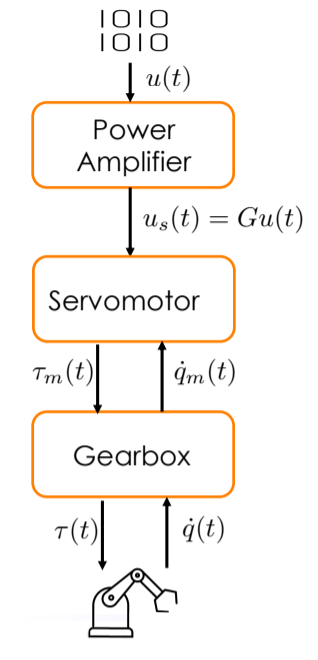
\includegraphics[width=\linewidth]{imgs/control_process_with_servomotors.png}
  \caption{Control process with servomotors.}
\end{wrapfigure}


The control process starts from digital information provided by the controller; this information $u(t)$ represents the \textbf{control signals}. A \textbf{power amplifier} transforms them into a physical signal $u_s(t)=G\,u(t)$ to control the motor. The \textbf{servomotor} produces motion described by angular velocity $\dot{q}_m(t)$ and torque $\tau_m(t)$, which are transmitted through a \textbf{gearbox} adapting speed and torque to the mechanical structure. Finally, the robot joints experience angular velocity $\dot{q}(t)$ and torque $\tau(t)$, i.e., the \textbf{torque that moves the joints}. The input therefore comes as digital information from the controller, the servomotor generates torque and angular velocity, and the gearbox adapts this torque to effectively move the robot joints.

\hfill

\subsubsection*{DC Motors}

DC motors are \textbf{mainly designed to achieve high rotational speeds with low torques}.  
They are typically used in high-speed, high-volume industrial automation.  

\textit{Note: In industrial applications, we want to move as fast as possible.}

The angular position and velocity of the rotating axis can be measured using sensors:
\begin{itemize}
    \item Position $\rightarrow$ encoder
    \item Velocity $\rightarrow$ encoder (+processing) or resolver
    \item Torque/current $\rightarrow$ torque or current sensors
\end{itemize}

\textbf{Low-level position and velocity control is embedded} in servomotors.  

\textit{Note: The controller integrates the motor movement at the lowest input level.}

\hfill

\subsubsection*{Gearbox}

A \textbf{gearbox} is a mechanical device used to increase output torque or change motor speed.  

The motor shaft is connected to one end of the gearbox and, through the internal gear configuration, provides an output torque and a specific speed determined by the gear ratio.  

\[
\begin{cases}
t(t) = k t_m(t) \\
\omega_m(t) = k \, \omega(t)
\end{cases}
\]

with $k > 0$ the \textbf{gain of the gearbox}.  

From the equations it follows that:
\[
t(t)\,\omega(t) = t_m(t)\,\omega_m(t)
\]
that is, \textbf{power is preserved}.  

\textit{Notes:}  
\begin{itemize}
    \item The input is the motor’s angular velocity $\omega_m$ and torque $t_m$.  
    \item The output is the angular velocity $\omega$ and torque $t$.  
    \item Increasing torque implies decreasing velocity: \textit{more torque, but less velocity}.  
    \item These relations allow us to exchange torque and velocity according to the gear ratio.  
    \item This transformation maintains power balance.  
    \item Intuitively: more power and force can be achieved at the expense of speed, and vice versa.  
\end{itemize}

\hfill

\subsubsection*{Servomotors}

The use of servomotors in robotics requires \textbf{high torques}, for moving the links connected to the joints, but \textbf{lower speeds} with respect to the ones required in standard industrial automation applications.  

Gearboxes are exploited for achieving the right balance between speed and torque of the joints.  

\[
\begin{cases}
\tau(t) = K \tau_m(t) \\
\dot{q}_m(t) = K \dot{q}(t)
\end{cases}
\quad
K = 
\begin{pmatrix}
K_1 & 0   & \dots & 0 \\
0   & K_2 & \dots & 0 \\
\vdots & \vdots & \ddots & \vdots \\
0   & 0   & \dots & K_n
\end{pmatrix}, 
\quad K_i \gg 1
\]

The torque of the motors is amplified and the speed is attenuated.  

\textit{Notes:}  
\begin{itemize}
    \item $\tau$ is the output torque at the joint, $\tau_m$ is the torque of the motor.  
    \item $\dot{q}$ is the angular velocity of the joint, $\dot{q}_m$ is the angular velocity of the motor.  
    \item Since $K_i \gg 1$, we obtain much larger torque at the output, but lower angular velocity.  
    \item Power is preserved:  
    \[
    \tau = K \tau_m, \quad \dot{q}_m = K \dot{q}, \quad \Rightarrow \quad \tau^T \dot{q} = \tau_m^T \dot{q}_m
    \]  
    \item Intuitively: the gearbox amplifies the torque and reduces the velocity while maintaining the power balance.  
\end{itemize}

\hfill

\subsection{Actuation and Mechanics}

What is directly controlled is the input of the servomotors.  

The dynamics of the servomotors and the gain of the gearboxes have a strong impact on the system to be controlled.  

\[
M(q)\ddot{q} + C(q,\dot{q})\dot{q} + D\dot{q} + g(q) = \tau
\quad \text{(Euler-Lagrange equation)}
\]

\[
\begin{cases}
\tau(t) = K \tau_m(t) \\
\dot{q}_m(t) = K \dot{q}(t)
\end{cases}
\quad
K = 
\begin{pmatrix}
K_1 & 0   & \dots & 0 \\
0   & K_2 & \dots & 0 \\
\vdots & \vdots & \ddots & \vdots \\
0   & 0   & \dots & K_n
\end{pmatrix}, 
\quad K_i \gg 1
\]

The driving torque of each motor is controlled.  

The driving torque of the actuator produces a torque on the robot joint \textit{through the gearbox}.

\hfill

Combining the mechanics of the robot and the gearbox constitutive equations:

\[
M(q)\ddot{q} + C(q,\dot{q})\dot{q} + D\dot{q} + g(q) = \tau
\quad\quad
\begin{cases}
\tau(t) = K \tau_m(t) \\
\dot{q}_m(t) = K \dot{q}(t)
\end{cases}
\]

We get the dynamics of the variables at the motor side:

\[
K^{-1}M(q)K^{-1}\ddot{q}_m + K^{-1}C(q,\dot{q})K^{-1}\dot{q}_m + K^{-1}D K^{-1}\dot{q}_m + K^{-1} g(q) = \tau_m
\]

How?

Starting from Euler-Lagrange Model:

\[
M(q)\ddot{q} + C(q,\dot{q})\dot{q} + D(q,\dot{q})\dot{q} + g(q) = \tau
\]

Replacing $\big(q = K^{-1} q_m \big)$:

\[
M\!\left(K^{-1} q_m\right) K^{-1} \ddot{q}_m 
+ C\!\left(K^{-1} q_m, K^{-1}\dot{q}_m\right) K^{-1}\dot{q}_m 
+ D K^{-1}\dot{q}_m 
+ g\!\left(K^{-1} q_m\right) 
= K \tau_m
\]

\[
K^{-1} M(q_m) K^{-1} \ddot{q}_m 
+ K^{-1} C(q_m,\dot{q}_m) K^{-1}\dot{q}_m 
+ K^{-1} D K^{-1}\dot{q}_m 
+ K^{-1} g(q_m) 
= \tau_m
\]

\hfill

It is always possible to write the inertia matrix as:  

\[
M(q) = \bar{M} + \Delta M(q)
\]

where $\bar{M}$ is a constant diagonal matrix containing the average inertia at the joints and $\Delta M(q)$ contains the nonlinear terms of the inertia matrix.  

It is possible to write:

\[
\underbrace{K^{-1}\bar{M}K^{-1}\ddot{q}_m + K^{-1}D K^{-1}\dot{q}_m}_{\text{Linear}} 
\quad + \quad 
\underbrace{K^{-1}\Delta M(q)K^{-1}\ddot{q}_m + K^{-1}C(q,\dot{q})K^{-1}\dot{q}_m + K^{-1}g(q)}_{\text{Nonlinear}}
= \tau_m
\]

The nonlinear part is the most complex, but its effect can be attenuated by the following consideration.

Since the terms in $K$ are very big, the terms in $K^{-1}$ are very small. This brings to a big attenuation of the nonlinear terms of the model. Thus, it is possible to consider the nonlinear part of the model as a disturbance:  

\[
K^{-1}\bar{M}K^{-1}\ddot{q}_m + K^{-1}D K^{-1}\dot{q}_m = \tau_m - d(t)
\]

where all the matrices are constant and diagonal:

\[
K^{-1} =
\begin{pmatrix}
K_1^{-1} & 0 & \dots & 0 \\
0 & K_2^{-1} & \dots & 0 \\
\vdots & \vdots & \ddots & \vdots \\
0 & 0 & \dots & K_n^{-1}
\end{pmatrix},
\quad
\bar{M} =
\begin{pmatrix}
\bar{m}_1 & 0 & \dots & 0 \\
0 & \bar{m}_2 & \dots & 0 \\
\vdots & \vdots & \ddots & \vdots \\
0 & 0 & \dots & \bar{m}_n
\end{pmatrix},
\quad
D =
\begin{pmatrix}
d_1 & 0 & \dots & 0 \\
0 & d_2 & \dots & 0 \\
\vdots & \vdots & \ddots & \vdots \\
0 & 0 & \dots & d_n
\end{pmatrix}
\]

This leads to the following block structure (nonlinear coupled vs. linear decoupled):

\begin{figure}[H]
    \centering
    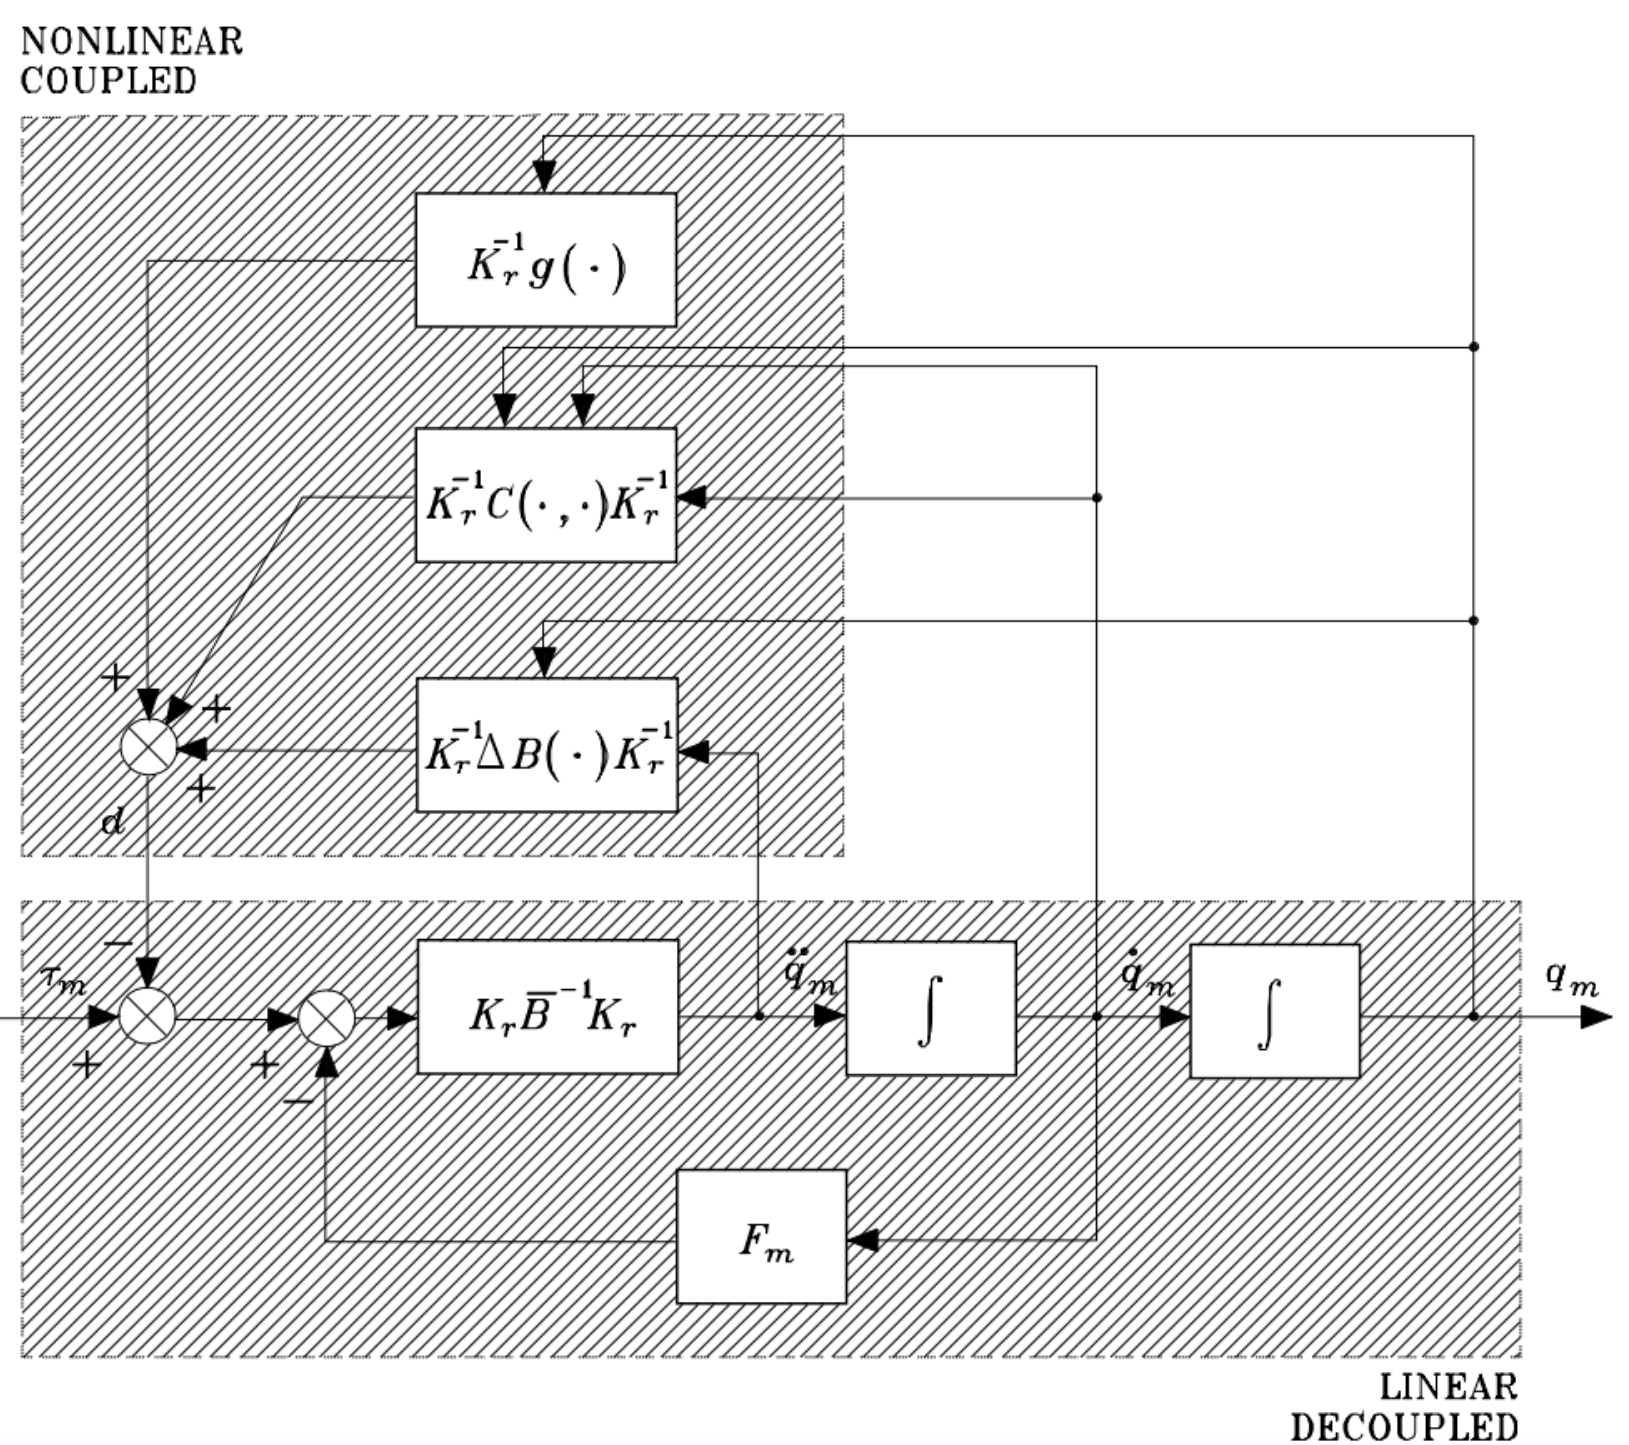
\includegraphics[width=\linewidth]{imgs/actuation_mechanics_block.png}
    \caption{Organization of the model into nonlinear coupled part and linear decoupled part.}
\end{figure}

In practice, we obtain a linear system for two reasons: we apply a mechanical reduction factor to the gearboxes ($K \gg 1$) and we reduce the disturbance through a linear control.

The system to control (by $\tau_m$) is a \textbf{linear and decoupled system with a disturbance}:

\[
\frac{\bar{m}_i}{k_i^2}\ddot{q}_{mi} + \frac{d_i}{k_i^2}\dot{q}_{mi} = \tau_{mi} + d_i(t), \quad i = 1,\dots,n
\]

Each joint can be considered as an independent SISO system with a linear dynamics.  

The dynamics can be represented as a transfer function, and the position/velocity of each joint can be controlled by standard control strategies with \textbf{high disturbance rejection}.  

Thanks to these techniques, the robots can be controlled either in velocity or in position.  

\[
\dot{q} \approx \dot{q}_d, \quad q \approx q_d
\]

\hfill

\subsubsection*{Position/Velocity Actuated Robots}

Since the control of each joint allows to achieve the desired joint velocity, the robot can be simply modeled by:

\[
\dot{q} = u 
\quad \longrightarrow \quad
v = J(q)\dot{q} 
\quad \longrightarrow \quad
v = u_c = J(q)u
\]

where $u = G_v v_c$, with $v_c$ the control voltage of the motor and $G_v$ the motor actuation constant.  

Controlling position/velocity actuated robots is simple since the specific choice of the actuation system \textit{“eliminates”} the nonlinear part of the robot.  

The system to be controlled becomes a simple set of decoupled SISO systems.

Many industrial robots are position/velocity controlled. \textit{Note: Here we are talking about servomotors + gearboxes.} 

PROs:
\begin{itemize}
    \item Simple to control (the nonlinear dynamics of the robot is strongly attenuated by the gearboxes).  
    \item Thanks to the amplification of the motor torque, the actuation through a gearbox allows to move large-size robots.  
\end{itemize}

CONs:
\begin{itemize}
    \item Velocity and acceleration are not too high because of the need to approximate the nonlinear dynamics as a disturbance.  
    \item Limited precision because of the presence of a disturbance.  
\end{itemize}

\hfill

\subsubsection*{Torque actuated robots}

If the required velocity and precision are high, the \textbf{direct drive actuation} is often preferred. The shaft of the motor is directly connected to the joint and no gearbox is present.

In this case, the current of the servomotor is controlled and the joint torque is given by:

\[
\tau = G v_c = u
\]

where $G$ is the current actuation constant and $v_c$ is the control voltage of the motor.

The model of the actuated robot is given by:

\[
M(q)\ddot{q} + C(q,\dot{q})\dot{q} + D\dot{q} + g(q) = u 
\quad \text{(Euler–Lagrange)}
\]

In the task space, this becomes:

\[
M_c(x)\ddot{x} + C_c(x,\dot{x})\dot{x} + D_c\dot{x} + g_c(x) = F_c
\]

with $x, \dot{x}, F_c \in \mathbb{R}^6$ and 
\[
\tau = J^T(q)F_c
\]

The control problem for torque actuated robots is more challenging than the control problem for velocity controlled robots.  

The system to control is nonlinear and coupled, and the linear control techniques learned in basic control courses are not directly applicable anymore.  

\hfill

Many last generation robots are torque controlled (e.g. collaborative robots).  

PROs:
\begin{itemize}
    \item High precision  
    \item High speed  
    \item Possibility of physically interacting with the user  
\end{itemize}

CONs:
\begin{itemize}
    \item Limited payload (due to the loss of torque amplification implemented by the gearbox).  
    \item More complex control.  
\end{itemize}

\hfill

\subsection*{Mobile Robots Actuation}

Low-level actuation of the wheels:

\begin{figure}[H]
    \centering
    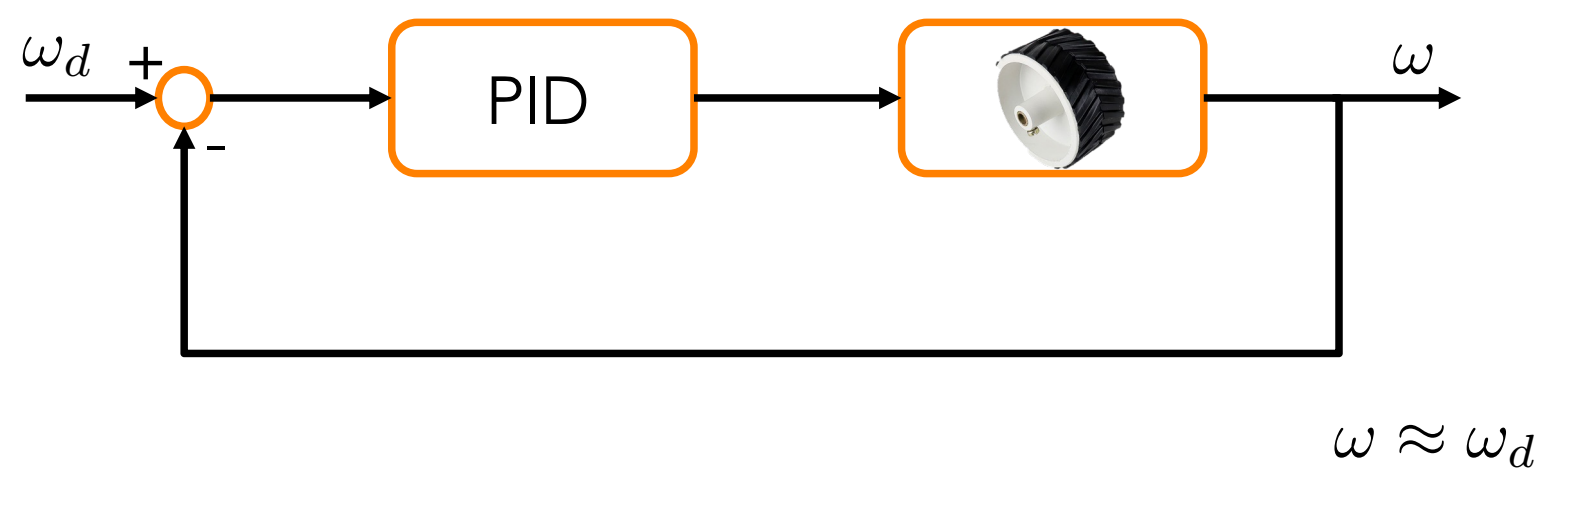
\includegraphics[width=0.75\linewidth]{imgs/low_level_actuation_of_wheels.png}
\end{figure}

This makes the model of the system kinematic.  

The speed setpoint for the wheels is obtained from the kinematic input of the robot.  

\textit{Note: With this approach, the angular velocity can be used as input, making the system a kinematic one.}

\hfill

\subsubsection{Robot Differential Drive}
\label{robot_differential_drive}

Two motors (one per wheel).  

It is equivalent to the unicycle. Kinematic inputs: $v$ and $\omega$.

\[
\begin{cases}
v = \dfrac{(\omega_R + \omega_L)r}{2} \\
\omega = \dfrac{(\omega_R - \omega_L)r}{d}
\end{cases}
\quad \Longrightarrow \quad
\begin{pmatrix}
\omega_R \\
\omega_L
\end{pmatrix}
=
\begin{pmatrix}
\dfrac{d}{r} & \dfrac{d}{2r} \\
\dfrac{1}{r} & -\dfrac{d}{2r}
\end{pmatrix}
\begin{pmatrix}
v \\
\omega
\end{pmatrix}
\]

where $r$ is the radius of the wheels and $d$ is the distance between the wheels.  

\hfill

\subsubsection{Robot Car-Like/Tricycle}

Two motors:
\begin{itemize}
    \item \textbf{Tractions:}
    \begin{itemize}
        \item Front wheel, or  
        \item Back wheels (with differential).  
    \end{itemize}
    \item \textbf{Steering:}
    \begin{itemize}
        \item Front wheel.  
    \end{itemize}
\end{itemize}

The kinematic inputs are directly mapped on the motor setpoints:
\begin{itemize}
    \item $v \;\; \rightarrow$ traction  
    \item $\omega \;\; \rightarrow$ steering  
\end{itemize}

\hfill

\subsection{Mobile Robots model}

The wheels of mobile robots are controlled by means of high-gain controllers.  

\begin{figure}[H]
    \centering
    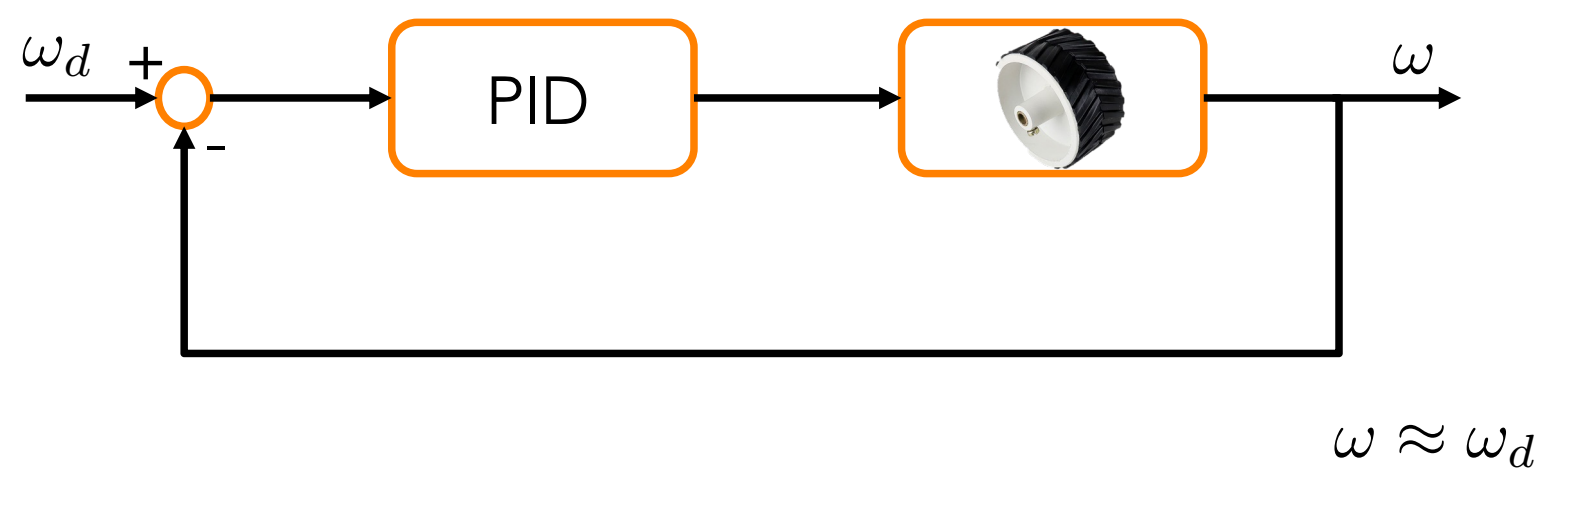
\includegraphics[width=0.75\linewidth]{imgs/low_level_actuation_of_wheels.png}
\end{figure}

The controller compensates the dynamics of the wheel.  

It is possible to command directly the speed of the robot and, therefore, the inputs of a mobile robot are often the velocities.  

The velocity inputs are also called \textbf{kinematic inputs}.  

The model of a mobile robot creates a relation between the kinematic inputs and the evolution of the configuration.

\hfill

\subsubsection{Model of a differential drive robot}

The differential drive robot is kinematically equivalent to a unicycle.  

\begin{figure}[H]
    \centering
    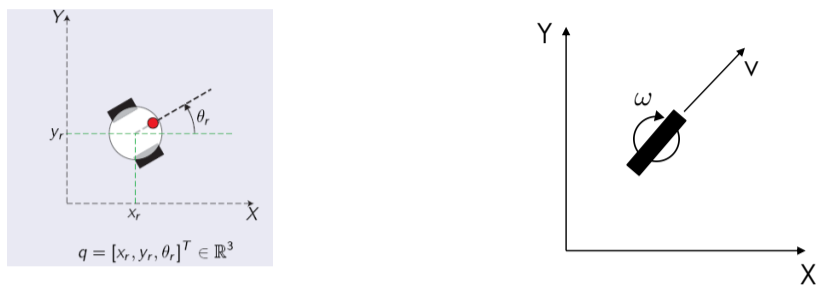
\includegraphics[width=1\linewidth]{imgs/diff_drive_unicycle.png}
\end{figure}

\textit{Note: $x_r, y_r, \theta_r$ are the configuration variables.}

Same basic motions: translations and rotation on the spot.  

The mid-point of the axis connecting the wheels is equivalent to the contact point of the wheel of the unicycle with the floor.  

The speed of the mid-point of the wheel axis $v$ and the angular velocity $\omega$ of the robot are linked one-to-one to the rotation speeds of the wheels:

\[
\begin{cases}
v = \dfrac{(\omega_R + \omega_L)r}{2} \\
\omega = \dfrac{(\omega_R - \omega_L)r}{d}
\end{cases}
\]

where:

\begin{itemize}
    \item $\omega_R$ = rotation speed of the right wheel  
    \item $\omega_L$ = rotation speed of the left wheel  
    \item $r$ = radius of the wheels  
    \item $d$ = distance between the wheels  
\end{itemize}

\textbf{Given a kinematic input $[v, \omega]$ to reproduce, it is always possible to find a pair $[\omega_R, \omega_L]$ that implements it.}  

\textit{Note: This generalizes the relations seen at paragraph \ref{robot_differential_drive}}

The kinematic model of the differential drive robot can be built by considering as kinematic inputs $[v, \omega]$ and the simpler structure of the unicycle.  

\hfill

A model can be obtained relating the derivatives of the configuration variables with the control variables:

\begin{figure}[H]
    \centering
    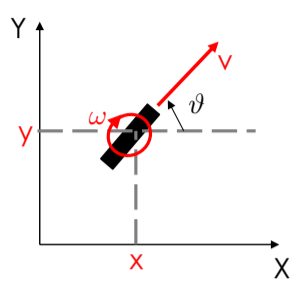
\includegraphics[width=0.35\linewidth]{imgs/unicycle.png}
\end{figure}

\[
\begin{cases}
\dot{x} = v \cos \vartheta \\
\dot{y} = v \sin \vartheta \\
\dot{\vartheta} = \omega
\end{cases}
\]

\textbf{Nonholonomic constraint:}
\[
\dot{x}^2 + \dot{y}^2 = v^2
\]

\textit{Notes:}
\begin{itemize}
    \item In this case, the constraint is both a velocity constraint (the robot cannot move instantaneously) and a direction constraint (the robot cannot move in a direction orthogonal to the velocity).
    \item This constraint is usually a non-integrable (non-solvable) second-order differential equation that tells us which movements the robot modeled with this model cannot make.
\end{itemize}

The translational velocities are constrained from the nonholonomic constraint introduced by the wheel: the robot cannot instantaneously move in a direction orthogonal to $v$. No constraints exist on the rotations.

The constraint does not limit the reachable configurations. Only the instantaneous mobility of the robot is limited.

\hfill

\subsubsection{Model of the tricycle and of the car-like robot}

The mobile robots with a tricycle or car-like structure are equivalent to a bicycle (\textit{Note: kinematically, not dynamically}).

\begin{figure}[H]
    \centering
    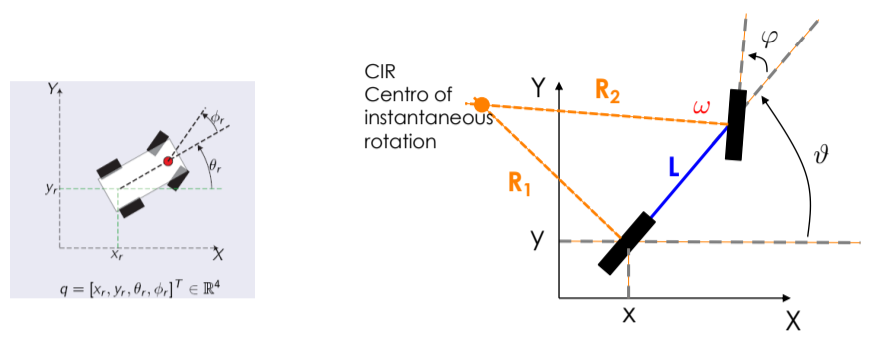
\includegraphics[width=1\linewidth]{imgs/tricycle_car_like_model.png}
\end{figure}

The bicycle cannot rotate on the spot. With a fixed steering angle, every wheel moves along an arc of a circle with center called the \textbf{center of instantaneous rotation (CIR)}.

$R_2$ is always greater than $R_1$, therefore the front wheel follows a longer path and rotates faster than the back wheel.  

If the steering angle is set to zero, the CIR goes to infinity and the bicycle moves along a straight line.  

\hfill

\subsubsection{Model of the bicycle with back traction}

\begin{figure}[H]
    \centering
    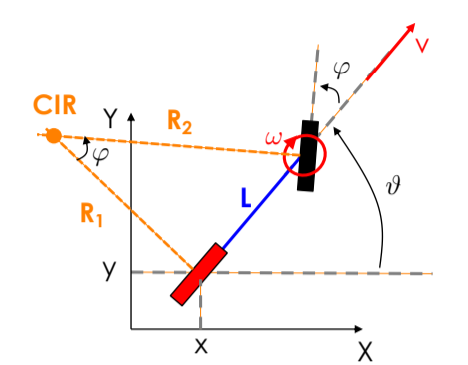
\includegraphics[width=0.5\linewidth]{imgs/bicycle_back_traction.png}
\end{figure}

The back wheel moves at the velocity $v$:  
\[
\dot{x} = v \cos \vartheta, \quad \dot{y} = v \sin \vartheta
\]
    
The back wheel moves instantaneously on a circle with radius $R_1$ and center CIR:  

\[
v = R_1 \dot{\vartheta} \quad \Rightarrow \quad \dot{\vartheta} = \frac{v}{R_1}
\]
    
$R_1$ changes over time and it is not an input or a configuration parameter of the robot: 

\[
R_2 \cos \varphi = R_1, \quad R_2 \sin \varphi = L \quad \Rightarrow \quad \tan \varphi = \frac{L}{R_1}
\]
    
The steering velocity influences only the steering angle:  
\[
\dot{\varphi} = \omega
\]

The model of the bicycle with back traction is:

\[
\begin{cases}
\dot{x} = v \cos \vartheta \\
\dot{y} = v \sin \vartheta \\
\dot{\vartheta} = \frac{v}{L} \tan \varphi \\
\dot{\varphi} = \omega
\end{cases}
\]

where:

\begin{itemize}
    \item $(v, \omega)$ are the kinematic inputs.  
    \begin{itemize}
        \item In tricycle/car-like robots, they represent traction and steering velocity.  
    \end{itemize}
    
    \item The mobility of the robot is instantaneously constrained.  
    \begin{itemize}
        \item Constraints act on the variation of the configuration variables.  
    \end{itemize}
\end{itemize}

\hfill

\subsubsection{Model of the bicycle with front traction}

The speed of the back wheel is $v \cos \varphi$:  

\[
\dot{x} = v \cos \varphi \cos \vartheta, \quad \dot{y} = v \cos \varphi \sin \vartheta
\]
    
The back wheel moves instantaneously on a circle with radius $R_1$ and center CIR:  

\[
v \cos \varphi = R_1 \dot{\vartheta} \quad \Rightarrow \quad \dot{\vartheta} = \frac{v \cos \varphi}{R_1}
\]
    
$R_1$ changes over time and is not an input or configuration parameter:  

\[
\tan \varphi = \frac{L}{R_1} \quad \Rightarrow \quad \dot{\vartheta} = \frac{v}{L} \tan \varphi
\]
    
Steering velocity influences only the steering angle:  
\[
\dot{\varphi} = \omega
\]

\hfill

The model of the bicycle with front traction is

\[
\begin{cases}
\dot{x} = v \cos \varphi \cos \vartheta \\
\dot{y} = v \cos \varphi \sin \vartheta \\
\dot{\vartheta} = \frac{\sin \varphi}{L} v \\
\dot{\varphi} = \omega
\end{cases}
\]

where:

\begin{itemize}
    \item $(v, \omega)$ are the kinematic inputs.  
    \begin{itemize}
        \item In tricycle/car-like robots, they represent traction and steering velocity.  
    \end{itemize}
    
    \item The mobility of the robot is instantaneously constrained.  
    \begin{itemize}
        \item Constraints act on the variation of the configuration variables.  
    \end{itemize}
\end{itemize}

\hfill

\subsection{Models recap}

\begin{figure}[H]
    \centering
    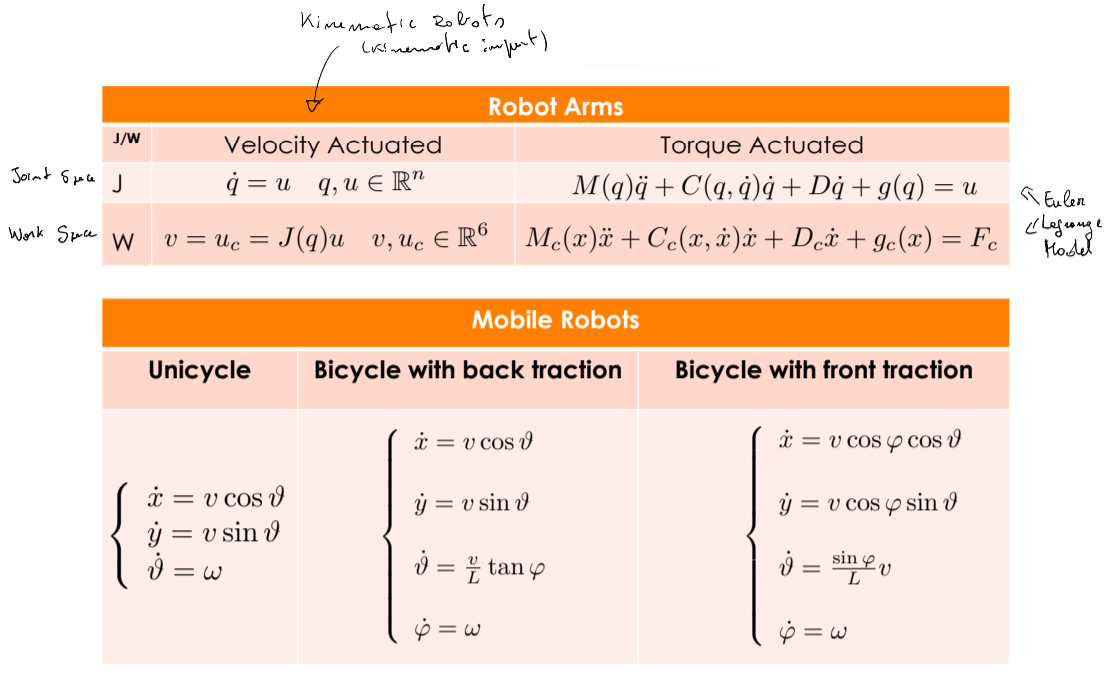
\includegraphics[width=1\linewidth]{imgs/models_recap.png}
\end{figure}

\hfill

\subsection{Control Architecture – Robotic Arms}

When dealing with robotic arms, the control objectives are typically defined in the \textbf{task space}, for example specifying the desired pose of the end-effector. However, both measurements (such as joint positions and velocities) and actuation signals (torques, positions, or velocities applied at the joints) are naturally expressed in the \textbf{joint space}. This creates a fundamental gap between where goals are defined and where control actions can be applied.  
To solve this problem, it is necessary to exploit the kinematic relations between the joint space and the task space.

\subsubsection*{Control in the Joint Space}

\begin{figure}[H]
    \centering
    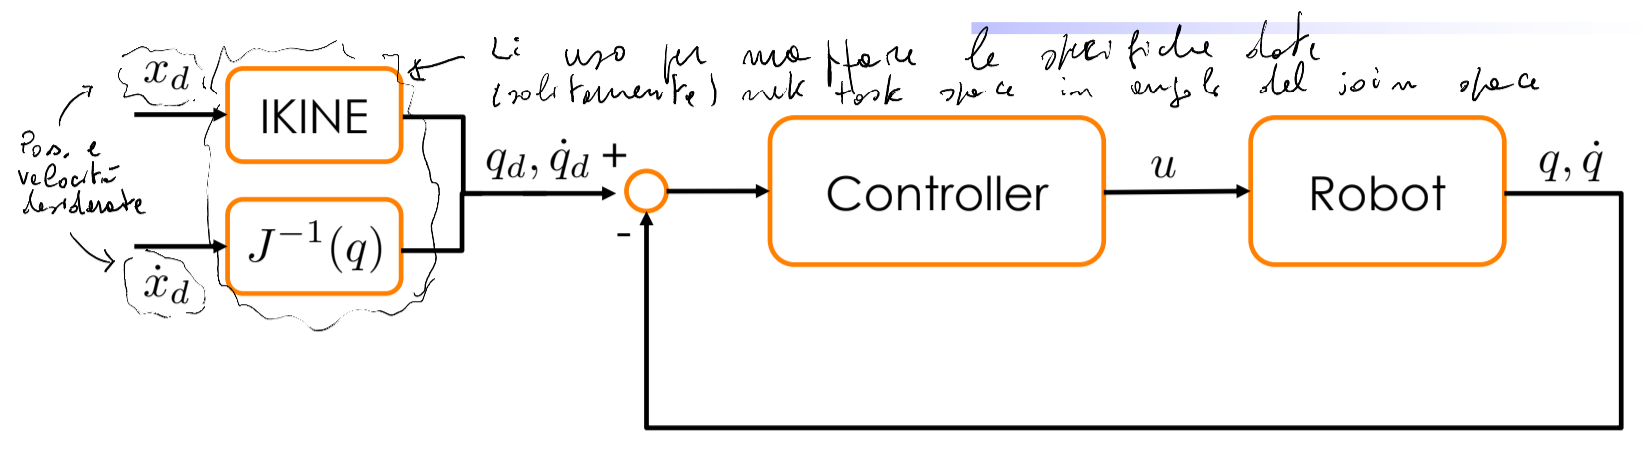
\includegraphics[width=1\linewidth]{imgs/control_joint_space_robotic_arms.png}
\end{figure}

A common strategy consists in expressing the setpoint directly in the joint space. This is obtained by applying \textbf{inverse kinematics}, which allows the mapping of desired quantities given in the task space into the joint space. The main difficulty in this approach lies in solving the inverse kinematics problem, since it may present singularities or multiple solutions, and must therefore be carefully handled during motion planning.  

In some particular cases, such as posture control, the setpoint can be directly specified in the joint space, and in this situation no inverse kinematics is required.

\subsubsection*{Control in the Workspace}

An alternative strategy is to build the controller directly in the task space. In this approach, the desired motion in the workspace is used as the setpoint, and the control loop is designed in terms of workspace variables. 

\begin{figure}
    \centering
    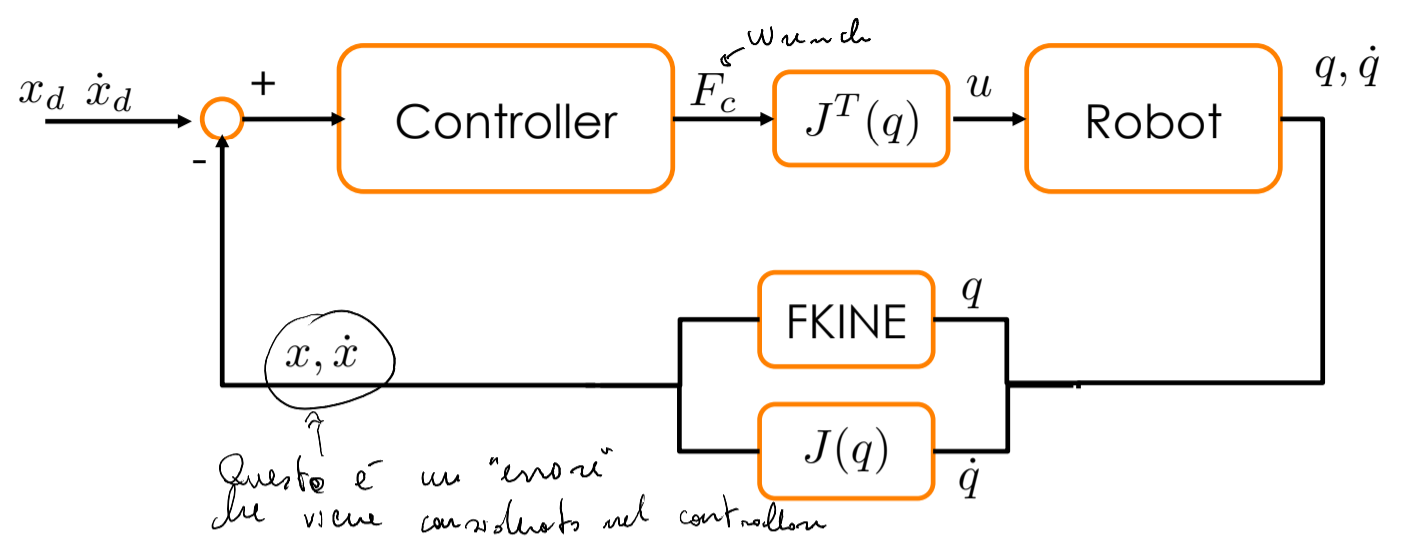
\includegraphics[width=1\linewidth]{imgs/control_work_space_robotic_arms.png}
\end{figure}

The measures obtained in the joint space must be transformed into workspace quantities, and the control input computed in the task space has then to be mapped back to the joint space.  

While this method allows a more direct specification of motion objectives, it requires a significantly higher computational effort compared to joint space control, since a large number of transformations and calculations have to be performed in real time.  

\hfill

\subsection{Control Architecture – Mobile Robots}

In mobile robots, the control architecture is typically organized in a \textbf{hierarchical structure}, with different control layers responsible for different aspects of the motion.

\begin{figure}[H]
    \centering
    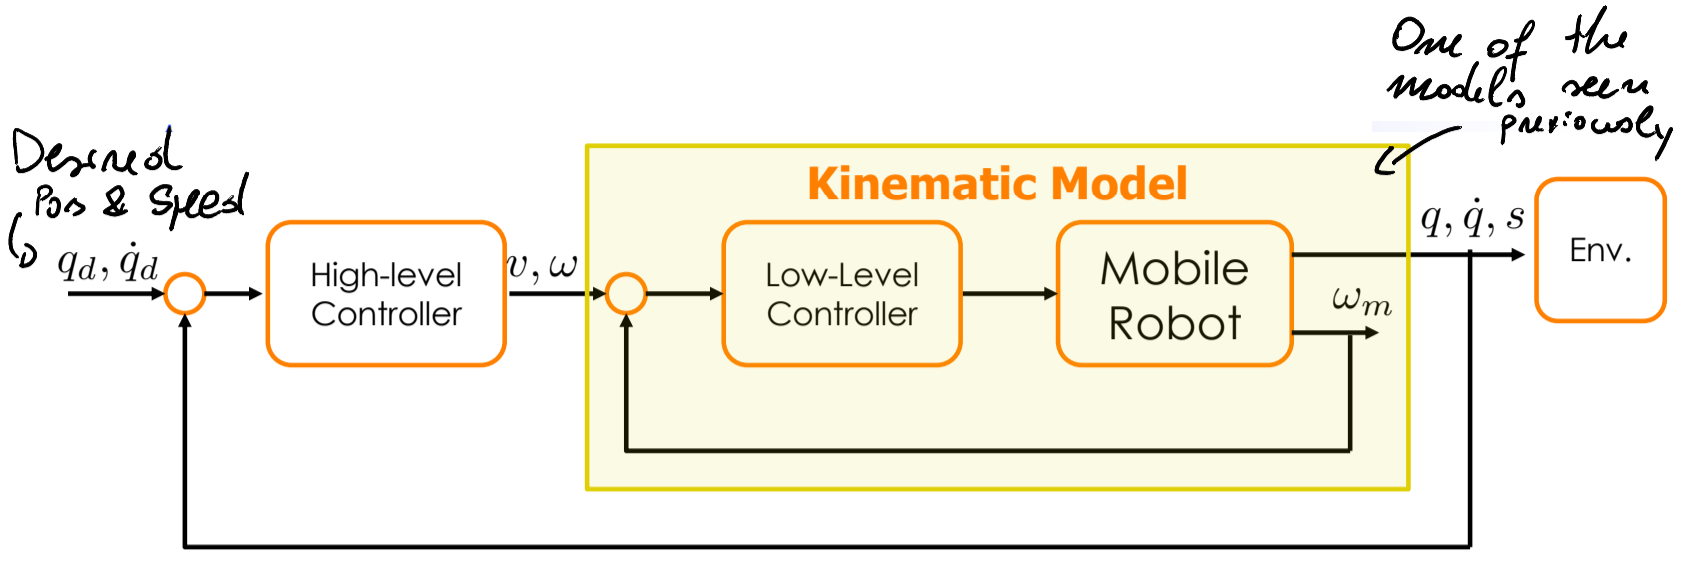
\includegraphics[width=1\linewidth]{control_mobile_robots.png}
\end{figure}

\subsubsection*{Low-level Control}
The low-level control regulates the speed of the wheels, effectively making the real robot equivalent to its kinematic model.  
Starting from the desired kinematic inputs, the corresponding rotating speed for each wheel is computed. By exploiting the feedback of wheel speeds, measured by \textbf{proprioceptive sensors}, a high-gain controller (such as a PID) ensures accurate tracking of the desired velocities.  

In this way, the influence of the wheel dynamics is compensated, and the low-level controller enforces the robot to follow the expected kinematic behavior.

\subsubsection*{High-level Control}
The high-level control regulates the overall motion of the robot with respect to its surrounding environment.  
Starting from the desired motion, and considering the kinematic model of the robot, the pose of the robot relative to the environment is estimated through \textbf{exteroceptive sensors} (e.g., vision systems). Based on this information, the high-level controller determines the kinematic inputs that the robot must follow to achieve the desired trajectory.  

This hierarchical structure separates the problem of wheel actuation (handled at low level) from the problem of global navigation and interaction with the environment (handled at high level).

\hfill

\subsection{Planning and Motion Control}

\begin{figure}
    \centering
    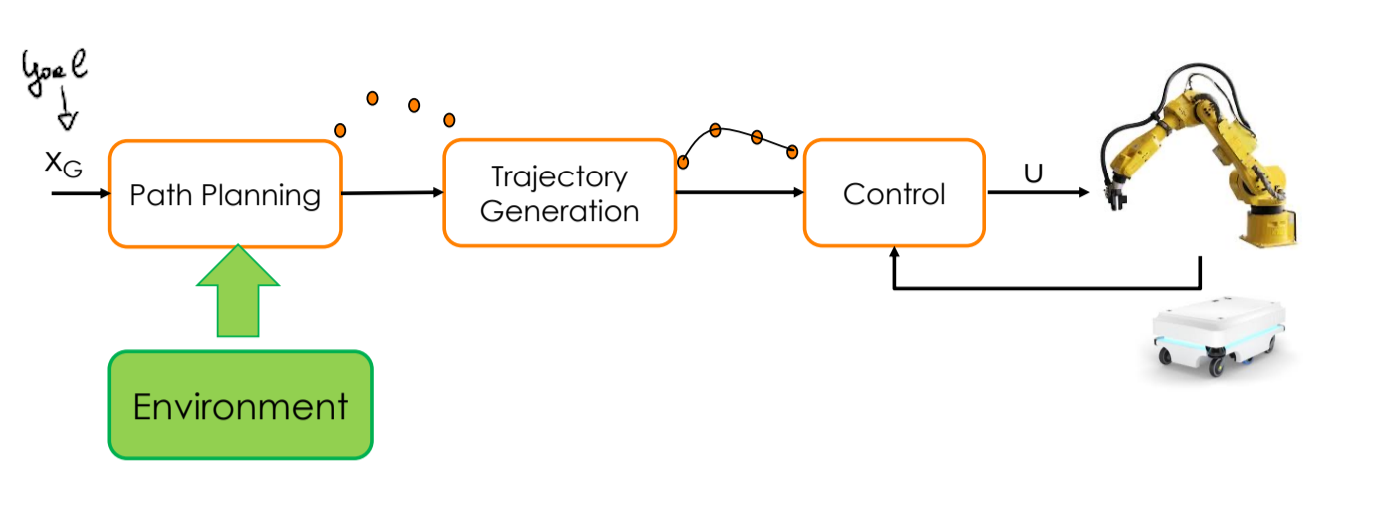
\includegraphics[width=1\linewidth]{imgs/planning_and_motion_control.png}
\end{figure}

In the control of robotic systems, planning and motion control play a crucial role.  
Given an objective, and possibly some information about the environment, it is first necessary to plan a collision-free path. From this path, a trajectory to execute is then generated, and finally a feedback controller guarantees good tracking of the desired trajectory.  
In other words, the planning and trajectory generation must be carried out carefully, and the entire responsibility cannot be delegated to the controller.

\subsubsection*{Planning}
Planning is fundamental when the robot moves in environments populated by obstacles, either static or dynamic.  
If the robot instead operates in an environment free from obstacles, such as a workcell, the trajectory can be directly generated without the need for complex planning.

\subsubsection*{Trajectory Generation}
Trajectory generation is necessary to set the time parameterization of the motion and to produce a setpoint that is compatible with the control frequency of the robot.

\subsubsection*{Control}
The control phase is fundamental to achieve the desired performance and to guarantee disturbance rejection.  
At this stage, the feedback controller ensures that the system follows the desired trajectory while compensating for uncertainties and external disturbances.

\hfill

\subsection*{Take Home Message}

The actuation system of a robot can have a significant impact on the final model that must be considered for control purposes.  
Moreover, the choice of the control architecture strongly influences the design of the controller. For robotic arms, this often means deciding whether to work in the joint space or in the workspace, while for mobile robots it may require the use of dynamic compensation.  

Finally, it is important to highlight that the model of the robot is crucial not only for planning tasks but also for the actual control of the robot itself.

